\documentclass[10pt, a4paper]{article}

%%%%%%%%%%%%%%
%  Packages  %
%%%%%%%%%%%%%%


\usepackage{page_format}
\usepackage{special}
\usepackage{hyperref}
\usepackage{tikz}
\usepackage[compat=1.1.0]{tikz-feynman}
\usepackage[font=small,labelfont=bf,
   justification=justified,
   format=plain]{caption}
%----------------------------------------------------------------------
%\usepackage{amssymb} % Mathematical fonts.
%\usepackage{amsfonts} % Mathematical fonts.
\usepackage[nice]{nicefrac} % Nicer fractions
\usepackage{braket} % Dirac Notation.
\usepackage{bbm} % More bold fonts.
%\usepackage{mathrsfs} % Mathematical fonts.
\usepackage{esint} % Integrals
\usepackage{cancel} % Allows to scratch expressions.
\usepackage{mathtools} % Tools for math formating.
\usepackage{slashed} % Allows to slash individual characters.
\usepackage{xargs} % Better handling of optional arguments for commands
%----------------------------------------------------------------------
%\usepackage{lmodern} % Fonts.
\usepackage{feyn} % Feynman Diagrams in mathmode

%%%%%%%%%%%%%%%%%%%%%%%%%%%
% Mathématiques et physique
%%%%%%%%%%%%%%%%%%%%%%%%%%%%
% SI Units -----------------------
% The package 'siunitx' causes unresolved crashes (as of 22/08/31)
\newcommand{\ampere}{\text{A}}
\newcommand{\bell}{\text{B}}
\newcommand{\celsius}{\degree\text{C}}
\newcommand{\coulomb}{\text{C}}
\newcommand{\degree}{\,^{\circ}}
\newcommand{\farad}{\text{F}}
\newcommand{\electro}{\text{e}}
\newcommand{\gram}{\text{g}}
\newcommand{\henry}{\text{H}}
\newcommand{\hertz}{\text{Hz}}
\newcommand{\hour}{\text{h}}
\newcommand{\joule}{\text{J}}
\newcommand{\kelvin}{\text{K}}
\newcommand{\meter}{\text{m}}
\newcommand{\minute}{\text{m}}
\newcommand{\mole}{\text{mol}}
\newcommand{\newton}{\text{N}}
\newcommand{\ohm}{\Omega}
\newcommand{\pascal}{\text{Pa}}
\newcommand{\rad}{\text{rad}}
\newcommand{\second}{\text{s}}
\newcommand{\tesla}{\text{T}}
\newcommand{\torr}{\text{Torr}}
\newcommand{\volt}{\text{V}}
\newcommand{\watt}{\text{W}}
%
\newcommand{\tera}{\text{T}}
\newcommand{\giga}{\text{G}}
\newcommand{\mega}{~\text{M}}
\newcommand{\kilo}{~\text{k}}
\newcommand{\deci}{\text{d}}
\newcommand{\centi}{\text{c}}
\newcommand{\milli}{\text{m}}
\newcommand{\micro}{\mu}
\newcommand{\nano}{\text{n}}
\newcommand{\pico}{\text{p}}
\newcommand{\femto}{\text{f}}
%
\newcommand{\units}[1]{\text{#1}}
\newcommand{\tothe}[1]{\textsuperscript{#1}}
%
\newcommand{\per}{\text{/}}
%
\newcommand{\Time}[3]{#1\hour~#2\minute~#3\second} % TODO Optional arguments.
\newcommand{\Angle}[3]{#1^{\circ}~#2'~#3''} % TODO Optional arguments.


% Better epsilon -----------------------
\let\oldepsilon\epsilon
\let\epsilon\varepsilon
\let\varepsilon\oldepsilon


% Better \bar -----------------------
\renewcommand{\bar}[1]{\mkern 1.5mu\overline{\mkern-1.5mu#1\mkern-1.5mu}\mkern 1.5mu}


% Équations -----------------------
\newcommand{\al}[1]{\begin{align} #1 \end{align}} % Numbered equation(s),
\newcommand{\eqn}[1]{\begin{align*} #1 \end{align*}} % Number-less equation(s),
\newcommand{\sys}[1]{\begin{dcases*} #1 \end{dcases*}} % System of equations.


% Exponents -----------------------
\newcommand{\Exp}[1]{\text{e}^{#1}}		% e^#
\newcommand{\E}[1]{\times 10^{#1}}		% X 10^#


% Delimiters -----------------------
\newcommand{\p}[1]{\left( #1 \right)}	% (#)
\newcommand{\cro}[1]{\left[ #1 \right]}	% [#]
\newcommand{\abs}[1]{\left| #1\right|}	% |#|
\newcommand{\avg}[1]{\left\langle #1 \right\rangle} % <#>
\newcommand{\acc}[1]{\left\lbrace #1 \right\rbrace} % {#}


% Vectors -----------------------
\newcommand{\ve}[1]{\mathbf{#1}} % Upright bold face.
\newcommand{\vu}[1]{\hat{\ve{#1}}} % Hat vector upright bold face
\newcommand{\tens}{\otimes} % Tensor product
\newcommand{\nablav}{\bm{\nabla}} % Bold gradient


% Trig. functions with automatic formating  -----------------------
\newcommandx{\Sin}[2][1={}]{\text{sin}^{#1}\!\p{#2}}
\newcommandx{\Cos}[2][1={}]{\text{cos}^{#1}\!\p{#2}}
\newcommandx{\Tan}[2][1={}]{\text{tan}^{#1}\!\p{#2}}
\newcommandx{\Csc}[2][1={}]{\text{csc}^{#1}\!\p{#2}}
\newcommandx{\Sec}[2][1={}]{\text{sec}^{#1}\!\p{#2}}
\newcommandx{\Cot}[2][1={}]{\text{cot}^{#1}\!\p{#2}}
\newcommandx{\Arcsin}[2][1={}]{\text{arcsin}^{#1}\!\p{#2}}
\newcommandx{\Arccos}[2][1={}]{\text{arccos}^{#1}\!\p{#2}}
\newcommandx{\Arctan}[2][1={}]{\text{arctan}^{#1}\!\p{#2}}
\newcommandx{\Sinh}[2][1={}]{\text{sinh}^{#1}\!\p{#2}}
\newcommandx{\Cosh}[2][1={}]{\text{cosh}^{#1}\!\p{#2}}
\newcommandx{\Tanh}[2][1={}]{\text{tanh}^{#1}\!\p{#2}}


% Matrices -----------------------
\newcommand{\mat}[1]{\begin{bmatrix} #1 \end{bmatrix}} % Matrices with hooks.
\newcommand{\pmat}[1]{\begin{pmatrix} #1 \end{pmatrix}} % Matrices with parentheses.
\newcommand{\deter}[1]{\abs{\begin{matrix} #1 \end{matrix}}} % Determinant.
\newcommandx{\mO}[2][1={}, 2={}]{ \def\temp{#2}\ifx\temp\empty\ve{O}_{#1}\else\ve{O}_{#1\times #2}\fi}% Zero matrix.
\newcommandx{\mI}[2][1={}, 2={}]{ \def\temp{#2}\ifx\temp\empty\ve{I}_{#1}\else\ve{O}_{#1\times #2}\fi}%  Identity matrix.
\newcommand{\Det}[1]{\text{det}\p{#1}} % det(#)
\newcommand{\Tr}[1]{\text{Tr}\p{#1}} % Tr(#)


% Derivatives -----------------------
\newcommand{\D}{\text{d}} % Differential 'd'.
\newcommandx{\dd}[3][1={},3={}]{\frac{\D^{#3}#1}{\D{#2}^{#3}}} % Total derivative according to #2, #1 is the function and #3 is the order.
\newcommand{\del}{\partial} % Partial 'd'.
\newcommandx{\ddp}[3][1={},3={}]{\frac{\del^{#3}#1}{\del{#2}^{#3}}} % Dérivée partielle selon #2, #1 est la fonction est #3 est l'ordre.
\newcommand{\eval}[1]{\left. {#1} \right|} % Bar on the right of expression.
\newcommand{\delbar}{\slashed{\del}} % Partial Inexact differential.
\newcommand{\dbar}{\dj}% Inexact differential.


% Integrals -----------------------
\newcommand{\intinf}{\int\displaylimits_{-\infty}^{\infty}} % From -00 to 00.
\newcommandx{\Int}[2][1={},2={}]{\int\displaylimits_{#1}^{#2}} % Faster bounded integrals.


% Complex numbers -----------------------
\renewcommand{\Re}[1]{\text{Re}\acc{#1}} % Re{#}
\renewcommand{\Im}[1]{\text{Im}\acc{#1}} % Im{#}


% Sets -----------------------
\newcommand{\N}{\mathbbm{N}} % Natural numbers.
\newcommand{\Z}{\mathbbm{Z}} % Integers.
\newcommand{\Q}{\mathbbm{Q}} % Rational numbers.
\newcommandx{\R}[1][1={}]{\mathbbm{R}^{#1}} % Real numbers.
\newcommandx{\C}[1][1={}]{\mathbbm{C}^{#1}} % Complex numbers.
\newcommandx{\F}[1][1={}]{\mathbbm{F}^{#1}} % Some field.
\newcommand{\M}[3]{\mathbb{M}_{#1\times#2}(#3)}	% Matrices.
\newcommand{\Po}[2]{\mathbb{P}_{#1}(#2)} % Polynomials.
\newcommand{\Lin}{\mathbb{L}} % Linear maps.


% Constants and physical symbols -----------------------
\newcommand{\eo}{\epsilon_0} % epsilon 0.
\renewcommand{\L}{\mathcal{L}} % Lagrangian.

\usepackage{listings,xcolor}

% Default fixed font does not support bold face
\DeclareFixedFont{\ttb}{T1}{txtt}{bx}{n}{12} % for bold
\DeclareFixedFont{\ttm}{T1}{txtt}{m}{n}{12}  % for normal

\lstset{language=Mathematica}
\lstset{basicstyle={\sffamily\footnotesize},
  numbers=left,
  numberstyle=\tiny\color{gray},
  numbersep=5pt,
  breaklines=true,
  captionpos={t},
  frame={lines},
  rulecolor=\color{black},
  framerule=0.5pt,
  columns=flexible,
  tabsize=2
}

\usepackage{color}
\definecolor{deepblue}{rgb}{0,0,0.5}
\definecolor{deepred}{rgb}{0.6,0,0}
\definecolor{deepgreen}{rgb}{0,0.5,0}

\newcommand\pythonstyle{\lstset{
language=Python,
basicstyle=\ttm,
morekeywords={self},              % Add keywords here
keywordstyle=\ttb\color{deepblue},
emph={MyClass,__init__},          % Custom highlighting
emphstyle=\ttb\color{deepred},    % Custom highlighting style
stringstyle=\color{deepgreen},
frame=tb,                         % Any extra options here
showstringspaces=false
}}

\lstnewenvironment{python}[1][]
{
\pythonstyle
\lstset{#1}
}
{}


% References
\usepackage{biblatex}
\addbibresource{ref.bib}


%%%%%%%%%%%%
%  Colors  %
%%%%%%%%%%%%
% ! EDIT HERE !
\colorlet{chaptercolor}{red!70!black} % Foreground color.
\colorlet{chaptercolorback}{red!10!white} % Background color


%%%%%%%%%%%%%%
% Page titre %
%%%%%%%%%%%%%%
\title{Homework 1 : Equivalence principle at
work: charge in a lab} % Title of the assignement.
\author{\PA} % Your name(s).
\teacher{David Kubiznak and Ghazal Geshnizjani} % Your teacher's name.
\class{Relativity} % The class title.

\university{Perimeter Institute for Theoretical Physics} % University
\faculty{Perimeter Scholars International} % Faculty
%\departement{<Departement>} % Departement
\date{\today} % Date.


%%%%%%%%%%%%%%%%%%%%%%
% Begin the document %
%%%%%%%%%%%%%%%%%%%%%%
\begin{document}



% Make the title page.
\maketitlepage

% Make table of contents
\maketableofcontents

% Assignment starts here ----------------------------

\section{Uniformly accelerated charge}
Consider a charged particle of mass $m_0$ and charge $Q$ in a uniform constant electric field of magnitude $E$ aligned with the $x$ axis of an inertial frame associated with the cylindrical coordinate system $x^\mu = (t, x, \rho, \varphi)$ with spacetime interval $d s^2=-d t^2+d x^2+d \rho^2+\rho^2 d \varphi^2$. 
\begin{enumerate}
  \item[(a)] Denoting $u^{\mu}$ the four-velocity of the particle and $F^{\mu\nu}$ ($-E = F_{01} = -F_{10}$ and all other components are $0$) the Faraday tensor in the inertial coordinate system, we can write the relativistic second law with $k=Q / m_0$ as follows: 
  \begin{align*}
    \frac{d u_\mu}{d \tau}=k F_{\nu\mu} u^\nu &\iff 
    \begin{cases}
      \frac{d u_0}{d \tau}=k F_{\nu 0} u^\nu= k F_{1 0} u^1 = kE u^1,\\
      \frac{d u_1}{d \tau}=k F_{\nu 1} u^\nu = k F_{0 1} u^0 = -kE u^{0},\\
      \frac{d u_2}{d \tau}=k F_{\nu 2} u^\nu = 0,\\
      \frac{d u_3}{d \tau}=k F_{\nu 3} u^\nu = 0
    \end{cases}
    \iff 
    \begin{cases}
      \frac{d u^0}{d \tau} = -kE u^1,\\
      \frac{d u^1}{d \tau} = -kE u^{0},\\
      \frac{d u^2}{d \tau}= 0,\\
      \frac{d u^3}{d \tau} = 0.
    \end{cases}
  \end{align*} 
  Supposing the four-velocity components $u^2, u^3$ are $0$ at $\tau = 0$, the last two equations imply that they stay $0$ for all future times. The first two equations can be added/subtracted to get 
  \begin{align*}
    &\frac{d (u^0 + u^{1})}{d \tau} = -kE (u^{0} + u^1) \impliedby u^{0} + u^1 = A e^{-kE \tau},\  A\in \mathbb{R}\\
    &\frac{d (u^1-u^{0})}{d \tau} = kE (u^1 - u^{0}) \impliedby u^{1} - u^0 = B e^{kE \tau},\ B\in \mathbb{R}.
  \end{align*}
  wich combine into $u^0 = (A e^{-kE \tau} - B e^{kE \tau})/2$ and $u^1 = (A e^{-kE \tau} + B e^{kE \tau})/2$. The constants $A,B$ are fixed by taking $u^0 = 1,\ u^1 = 0$ at $\tau = 0$ (the charge is at rest in the lab frame at $\tau=0$) which leads to the solution $u^0 = \cosh(kE \tau),\ u^1 = \sinh(kE \tau)$. Integrating with respect to proper time, we get the following proper time parametrized trajectory of the charge:
  \begin{align*}
    t_Q = \dfrac{1}{kE}\sinh(kE \tau), \quad x_Q = \dfrac{1}{kE}\cosh(kE \tau),\quad \rho_Q = 0\quad \& \quad \varphi_Q = 0
  \end{align*}
  where we have supposed the particle is at, $x_Q = (kE)^{-1},\ \rho_Q = 0,\ \varphi = 0$ (a more careful treatment would not place the particle in the singular axis of our coordinate system where the chart map is degenerate, but here the dynamics of the particle can be extended to these degenerate points) and $t_Q = 0$ (clock synchronized with lab clock) at $\tau = 0$.
  \item[(b)] The general definition of the four-acceleration in non-cartesian coordinates involves the Christoffel symbols of the coordinate system. However here the dynamics is restricted to the part of the coordinates that involves the cartesian coordinates $t, x$. We can therefore express the four-acceleration
  \begin{align*}
    a = \frac{d u_\mu}{d \tau}\frac{d u^\mu}{d \tau}=-\dfrac{(kE)^2}{kE}\sinh^2(kE \tau) + \dfrac{(kE)^2}{kE}\cosh^2(kE \tau) = kE
  \end{align*}
  which is constant (we have uniform acceleration).
  % Thanks to Thiago for the insight on the generalization of the four accelerations to arbitrary coordinates.
  \newpage
  \item[(c)] Trajectories for the same initial velocities but different $kE$ are represented and described in figure \ref{traj} (Left). 
  \begin{figure}
    \centering
    \begin{tikzpicture}
      \begin{axis}[
        restrict y to domain=-4:4,
        xmin=0, xmax=1,
        ymin=-0.5, ymax=0.5,
        axis lines=center,
        axis on top=true,
        domain=0:2.5,
        ylabel=$t$,
        xlabel=$x$,
        width=8cm,
        height=8cm,
        clip=true,
        yticklabel=\empty,
        xticklabel=\empty,
        ytick=\empty,
        xtick=\empty
        ]

        \draw (3/6,0)  circle[radius=2pt];
        \fill (3/6,0)  circle[radius=2pt];
        \draw[->, blue] (0,0.05) -- (3/6,0.05) node [label=right:{\footnotesize $(kE)^{-1}$}] {};
        \draw[->, blue] (5/6,0) -- (5/6, 0.25) node [label=above:{\footnotesize $u^{\mu}(0)$}] {};
      \newcommand{\nMAX}{5};
      %Below the red parabola is defined
      
      \foreach \n in {1, ..., \nMAX} 
        {
            \addplot [domain=-10:10, samples=200, black, variable=\x] ({\n * cosh(x)/6}, {\n * sinh(x)/6});
        }
        \addplot [domain=-5:5, samples=20, red, thick, variable=\x] ({x}, {x}) ;
        \addplot [domain=-5:5, samples=20, red, thick, variable=\x] ({x}, {-x});
        \node [label={[shift={(0.35,0.4)}]\textcolor{red}{\footnotesize $kE \to \infty$}}] {};

      \end{axis}
      \end{tikzpicture}
      \begin{tikzpicture}
        \begin{axis}[
          restrict y to domain=-4:4,
          xmin=-0.25, xmax=1,
          ymin=-0.5, ymax=0.5,
          axis lines=center,
          axis on top=true,
          domain=0:2.5,
          ylabel=$t$,
          xlabel=$x$,
          width=9.5cm,
          height=8cm,
          clip=true,
          yticklabel=\empty,
          xticklabel=\empty,
          ytick=\empty,
          xtick=\empty
          ]

        
        
        \newcommand{\nMAX}{5};
        
        \foreach \n in {1, ..., \nMAX} 
          {   

              \ifthenelse{\n = 3}{\addplot [domain=-10:10, samples=200, blue, ultra thick, variable=\x] ({\n * cosh(x)/6}, {\n * sinh(x)/6});}{\addplot [domain=-10:10, samples=200, black, variable=\x] ({\n * cosh(x)/6}, {\n * sinh(x)/6})}
              ;
          }


          \newcommand{\nMA}{5};
          \foreach \n in {0, ..., \nMA} 
          {   
              \ifthenelse{\n = 2}{\addplot [domain=0:10, samples=200, ultra thick, blue, variable=\x] ({x}, {\n/\nMA *x})}{\addplot [domain=0:10, samples=200, black, variable=\x] ({x}, {\n/\nMA *x});};
              \addplot [domain=0:10, samples=200, black, variable=\x] ({x}, {-\n/\nMA *x});
          }

          \draw (0.1+0.1, 0.15+0.1) -- (0.2+0.1, 0.25+0.1);
          \draw (0.1+0.1, 0.15+0.1) -- (0.0+0.1, 0.25+0.1);
          \draw (0.1+0.1, 0.15+0.1)  circle[radius=2pt];
          \fill (0.1+0.1, 0.15+0.1)  circle[radius=2pt];

          \addplot [domain=-5:5, samples=20, red, thick, variable=\x] ({x}, {x}) ;
          \addplot [domain=-5:5, samples=20, red, thick, variable=\x] ({x}, {-x});
          \node [label={[shift={(0.35,0.4)}]\textcolor{red}{\footnotesize $T \to \infty$}}] {};
          \node [label={[shift={(0.35,-0.5)}]\textcolor{red}{\footnotesize $T \to -\infty$}}] {};


          \node [label={[shift={(1-0.05,+0.5-0.2)}]\textcolor{red}{\footnotesize $\textcolor{blue}{T}$}}] {};

          \node [label={[shift={(1-0.35,+0.5-0.1)}]\textcolor{red}{\footnotesize $\textcolor{blue}{\overline{X}}$}}] {};

          

          \node [label={[shift={(0.1,-0.25)}]\textcolor{red}{II}}] {};
          \node [label={[shift={(0.1,+0.15)}]\textcolor{red}{I}}] {};

          \node [label={[shift={(-0.2,0.05)}]\textcolor{red}{III}}] {};
        \end{axis}
        \end{tikzpicture}
      \caption{(Left) Representation of trajectories for the uniformly accelerated charge at rest in the lab frame at $t=0$. Each trajectory corresponds to a different value of acceleration $kE$ decreasing from left to right (infinite acceleration corresponds to the red trajectory and coincides with light cone branches). The greater the acceleration, the faster (in time $t$) the trajectory approaches the speed of light. As opposed to uniformly accelerated non-relativistic particles which move on a parabola with unbounded velocity, the relativistic charge approaches the speed of light asymptotically as $\tau \to \infty$. For small values of $kE$, the trajectory can be approximated as a parabola for large amounts of time and the classical solution is recovered. (Right) Constant coordinate $X$, $T$ curves for the Rindle coordinate system seen from the lab frame       \label{traj}}

  \end{figure}
  \item[(d)] To describe the particle from the point of view of an observer accelerating with it, we use a new (Rindler) coordinate system $(T, X, \rho, \varphi)$ where $T$ is the proper time of a uniformly accelerated observer crossing the $x$ axis at $\overline{X} = X+(kE)^{-1}$ at $T=t=0$. We notice that the spacetime interval between the origin and any point on the accelerated trajectory $(\overline{X}\sinh(kE T), \overline{X}\cosh(kE T), 0, 0)$ (lab frame) is $\overline{X}$ (constant). So $\overline{X}$ represents the proper distance between the accelerated observer and the origin. Indeed the spacetime interval giving this distance is orthogonal (in the Lorentz sens) to the four-velocity along the hyperbolas and therefore links two simultaneous events in the instantaneous rest frame of the accelerated observer.
  
  A congruence of observers sweeping the left elsewhere of the origin can be formed by regrouping observers moving through all $X\in(-(kE)^{-1}, +\infty)$ with $T\in (-\infty, \infty)$ (light-like trajectories are not included since they are not parametrized by $T$). Expressing the lab coordinates in terms of the congruence coordinates, we get $$(t, x, \rho, \varphi) = (((kE)^{-1}+X)\sinh(kE T), ((kE)^{-1} + X)\cosh(kE T), \rho, \varphi).$$  Since $X$ represents a proper distance it can be extracted from the lab frame coordinates with the space-time interval $-t^2 + x^2 = \overline{X}^{2} $. The proper time $T$ is related to $x, t$ through a hyperbolic tangent as $\tanh(kE T) = t/x$. This indicates that constant $T$ curves are lines in the lab frame going through the origin. We note that the $x=0$ line coincides with constant proper time $T=0$ and lab time $t=0$ (clock synchronization). The constant coordinate lines of the Rindler frame are represented in the lab frame in figure \ref{traj} (Right). The observers only sweep a quarter of Minkowski spacetime. Any future light cone in region I$+$III has no overlap with the \textit{observed} region. This means that I$+$III can't influence the observers much like the content of the event horizon of a black hole. However, the observers can send signals to I (not to II and III). This is analogous to the fact we can enter black holes but to outside observers, the coordinate time at which we traverse is $T \to \infty$. Conversely, signals from region II can propagate to the observers from $T \to -\infty$,  but Rindler observers can never signal II$+$III. More formally, the outside of the Rindler observed regions, the events are not mapped to any coordinate and are not part of the chart used to describe an open subset of spacetime. The boundary of the observed region is light-like and not included in the chart (the subset of $\mathbb{R}^{1+1}$ is open) and constitutes event horizons. These horizons are present in absolute spacetime as light-like hypersurfaces but play a special role for the Rindler observer. To them, they are the end of observable spacetime. We can add that $\overline{X}<0$ is not relevant to our analysis because it produced a trajectory behind the previously described future and past horizons.
  \item[(e)] We can rewrite the Minkowski spacetime element in the Rindler coordinates as 
  \footnotesize{
  \begin{align*}
    ds^2  &= -dt^2 + dx^2 + d\rho^2 + \rho^2d\varphi^2 = -\left(\dfrac{\partial t}{\partial T} dT + \dfrac{\partial t}{\partial X} dX\right)^2 + \left(\dfrac{\partial x}{\partial T} dT + \dfrac{\partial x}{\partial X} dX\right)^2 + d\rho^2 + \rho^2d\varphi^2\\
    &= -\left((1+X (kE))\cosh(kE T)dT + \sinh(kE T) dX\right)^2 + \left((1 + X(kE))\sinh(kE T) dT + \cosh(kE T) dX\right)^2 + d\rho^2 + \rho^2d\varphi^2\\
    &= -(1+X (kE))^2\cosh^2(kE T)dT^2 - \sinh^2(kE T) dX^2 + (1 + X(kE))^2\sinh^2(kE T) dT^2 + \cosh^2(kE T) dX^2 + d\rho^2 + \rho^2d\varphi^2\\
    &= -(1+X (kE))^2dT^2 + dX^2 + d\rho^2 + \rho^2d\varphi^2.
  \end{align*}
  }

\end{enumerate}

\section{Field of a uniformly accelerated charge}
\begin{enumerate}
  \item[(a)] We turn to the calculation of the electromagnetic field sourced by the charge in the inertial lab frame. More precisely, we look for the four-potential with components $A^{\mu}$ solving the Maxwell wave equations in the Lorenz gauge (neglecting backreaction). The source term of the wave equation consists of a point charge $Q$ with proper time $\tau$ moving with four-velocity $u^{\mu}(\tau)$ on a trajectory $x^{\nu}_Q(\tau) = (t_Q, \mathbf{x}_Q)=  (t_Q(\tau), x_Q(\tau), 0, 0)$. At four-position $x^\nu = (t, \mathbf{x}) = (t, x, \rho, \varphi)$, the solution we look for is provided by the Lienard-Wiechert potential:
  % Do we neglect back reaction on the charge ?
  \begin{align*}
    A^\mu(x)=-\left.\frac{Q u^\mu(\tau)}{\left(x^\nu-x^\nu(\tau)_Q\right) u_\nu(\tau)}\right|_{\tau=\tau_r}
 \end{align*}
 where retarded proper time $\tau_r$ is the proper time at which a light ray received at $x^{\nu}$ is emitted from the charge. 
 
 If the emission and reception are connected by a light ray the associated spacetime interval vanishes and we have 
 \begin{align*}
  x^{\nu} - x^\nu_Q(\tau_r) = 0 \iff -(t-t_Q(\tau_r))^2+(\mathbf{x}-\boldsymbol{x}_Q)^2 = 0 \impliedby t = t_Q(\tau_r) + \sqrt{\rho^2 + (x-x_Q(\tau_r))^2}.
 \end{align*}
 where $t - t_Q(\tau_r)$ is taken to be positive so that the intersection of the \text{past light cone} ($t_Q(\tau_r) \leq t$) of $x^{\nu}$ with the hyperbolic trajectory of the charge is selected (the cause is in the past of the effect). This relation allows us to solve for $x_Q^{\mu}(\tau_r)$ associated with the retarded perception of the charge at $x^{\nu}$ (see item (c)). 
  \item[(b)] As shown above, the trajectory of a uniformly accelerated charge is given in cylindrical coordinates by
  \begin{align*}
    t_Q = \dfrac{1}{kE}\sinh(kE \tau), \quad x_Q = \dfrac{1}{kE}\cosh(kE \tau),\quad \rho_Q = 0\quad \& \quad \varphi_Q = 0. 
  \end{align*}
  Comparing the four-position with four-velocity leads to 
  \begin{align*}
    u^\mu = (\cosh(kE \tau),\ \sinh(kE \tau), 0, 0) = kE (x_Q, t_Q, 0, 0), \quad u_\mu = kE (-x_Q, t_Q, 0, 0).
  \end{align*}
  Substituting this expression of the four-velocity and the trajectory $x^\nu_Q$ in the Lienard-Wiechert potential yields
  \begin{align*}
    A^\mu(x)&=-\frac{Q}{\left(t-t_Q, x-x_Q, \rho, \varphi\right) \cdot kE (-x_Q, t_Q, 0, 0)} kE (-x_Q, t_Q, 0, 0)\\
    &=-\frac{Q}{- x_Q t+ x_Qt_Q + t_Qx-x_Qt_Q}  (-x_Q, t_Q, 0, 0)\\
    &=\frac{Q}{x_Q t - t_Q x}  (-x_Q, t_Q, 0, 0) = \frac{Q}{\xi}  (-x_Q, t_Q, 0, 0), \quad \text{with $\xi = x_Q t - t_Qx$}.
 \end{align*}
 where $t_Q, x_Q$ are evaluated at $\tau_r$.
  \item[(c)] From the retarded time's defining expression and the hyperbolic relation describing the trajectory of the charge, we can form the equations  
  \begin{align*}
    &x_Q^2 - t_Q^2 = \dfrac{1}{(kE)^2}\cosh^2(kE \tau) - \dfrac{1}{(kE)^2}\sinh^2(kE \tau) = \dfrac{1}{(kE)^2} = L^2 \\
    &0=-(t-t_Q)^2 + \rho^2 + (x-x_Q)^2 = - t^2 - t_Q^2 + 2t_Qt + \rho^2 + x^2+x_Q^2 - 2x x_Q \iff  -2t_Qt + 2x x_Q = \delta
  \end{align*}
  where $\delta = \rho^2 +x^2 + L^2 - t^2$. Combining this result with the definition of $\xi$ we have 
  \begin{align*}
    4\xi^2 - \delta^2 &= (2x_Q t - 2t_Qx)^2 - (2x x_Q-2t_Qt)^2 \\
    &= 4(x_Q^2 t^2 + t_Q^2 x^2 - 2 x_Q^2 t^2) - 4(x_Q^2 x^2 + t_Q^2 x^2 - 2 t_Q^2 t^2)\\
    &= 4x^2 (t_Q^2-x_Q^2) - 4t^2 (t_Q^2-x_Q^2) = 4L^2(x^2 - t^2)\\
    &\iff \xi^2 = (\delta^2-4L^2(x^2 - t^2 + \rho^2))/4 +\rho^2 L^2 = (L^2 + t^2 -\rho^2 -x^2)^2 + L^2\rho^2.
  \end{align*}
  showing that, like $\delta$, $\xi$ is independant of the unknowns $x_Q, t_Q$. This leaves us with the linear system of equations 
  
  \begin{align*}
    &\begin{cases}
      2\xi = 2x_Q t - 2t_Qx,\\
      \delta = -2t_Qt + 2x x_Q
    \end{cases}\\
    &\iff 
    \begin{cases}
      2\xi t - \delta x =  2x_Q t^2 - 2t t_Qx +2t_Qtx - 2x^2 x_Q = 2(t^2 - x^2) x_Q,  \\
      2\xi x - \delta t = 2x_Qx t - 2t_Qx^2 +2t_Qt^2 - 2x x_Q t = 2(t^2 - x^2) t_Q
    \end{cases}
    \iff 
    \begin{cases}
      x_Q = \dfrac{\delta x- 2\xi t}{2(x^2 - t^2)},  \\[0.3cm]
      t_Q = \dfrac{\delta t- 2\xi x}{2(x^2 - t^2)}. 
    \end{cases}
  \end{align*}

  % thanks to thiago for explaining the units 

  \item[(d)] The four-potential expression of the electromagnetic tensor is $F_{\mu \nu} = \partial_{\mu} A_{\nu} - \partial_{\nu} A_{\mu}$. Since the only non-zero components of $A_\mu$ are $A_0$, $A_1$  and depend only on $x^0, x^1, x^2$, the non trivial electromagnetic tensor components are $F_{01}, F_{02}, F_{12}$ (and their transpose). The $F_{01}, F_{02}$ components are associated to an electric field with components in the $x, \rho$ direction. The $F_{12}$ component is associated to a magnetic field curling around the $x$ axis in the $\varphi$ direction. 
\end{enumerate}

\section{Sitting on the charge}
\begin{enumerate}
  \item[(a)] The components of the four-vector potential found above are associated with an invariant vector field in spacetime. We can represent the components of this invariant object from the point of view of the Rindler observer accelerating with the charge. To acheive this transformation the expressions of $x^{\mu} = (x, t, \rho, \varphi)$ in terms of $X^{\mu} = (X, T, \rho, \varphi)$ are used to write $A_\mu$ as functions of $X, T$. Then the Rindler components are expressed as $A_\mu' = \frac{\partial x^\nu}{\partial X^{\mu}} A_\nu$ (from the invariant object perspective we have $A_\mu' dX^{\mu} = A_\mu dx^{\mu} =  \frac{\partial x^\nu}{\partial X^{\mu}} A_\nu dX^{\mu}$). The code below leads to the following result for the Rindler four-potential:
  \begin{align*}
    A_{\mu}' &= \left(-\Phi, \dfrac{-gQ}{gX+1}, 0, 0\right),\\
     &\text{with}\quad \Phi = \frac{Q \left(X^{2} g^{2} + 2 X g + \rho^{2} g^{2} + 2\right)}{g \sqrt{X^{4} + \frac{4 X^{3}}{g} + 2 X^{2} \rho^{2} + \frac{4 X^{2}}{g^{2}} + \frac{4 X \rho^{2}}{g} + \rho^{4} + \frac{4 \rho^{2}}{g^{2}}}} = \frac{Q \left(1 + X g + g^{2} r^2/2\right)}{r\sqrt{1 + g X + g^2 r^2/4}}\\
     &\text{and}  \quad r = \sqrt{\rho^2 + X^2}, \quad g = 1/L.
  \end{align*}
  The quantity $g$ represents gravitational field intensity existing in the non-inertial frame coaccelerating with the charge through the equivalence principle. We have a uniform electric field generating the acceleration and a gravitational field canceling it so the charge is static in the coaccelerating frame. 
  \begin{python}
import sympy as sp 

x, t, rho, phi, X, T, g, Q = sp.symbols(r"x t \rho \varphi X T g Q")

L = 1/g
xi = sp.sqrt((L**2 + t**2 - rho**2 - x**2)**2/4 + L**2 * rho**2)
delta = rho**2 + x**2 + L**2 - t**2

xQ = (x * delta - 2 * t * xi)/(2 * x ** 2 - 2 * t ** 2)
tQ = (t * delta - 2 * x * xi)/(2 * x ** 2 - 2 * t ** 2)

xc = (X+1/g) * sp.cosh(g * T)
tc = (X+1/g) * sp.sinh(g * T)

A = sp.Matrix([-xQ * Q/xi, tQ * Q/xi, 0, 0])
A.simplify()
A = A.subs({x : xc, t : tc})
A.simplify()

J = sp.Matrix([tc, xc, rho, phi]).jacobian([T, X, rho, phi]).T

ARindler = J * A
ARindler.simplify()
ARindler
  \end{python}
  \item[(b)] To simplify the four-potential found above we can perform a gauge transformation $A_\mu'' = A_\mu' + \partial_\mu \xi$ that will preserve the observable electric and magnetic fields. We choose $\xi$ to cancel the only non-zero component of $A_\mu'$ which corresponds to the equation 
  \begin{align*}
    0 = \dfrac{\partial \xi}{\partial X} + \dfrac{-gQ}{gX+1} \impliedby \xi = Q\ln(gX + 1) + 0. 
  \end{align*}
  The resulting four-potential is 
  \begin{align*}
    A_{\mu}'' &= \left(-\Phi + \frac{\partial 0}{\partial T}, \dfrac{-gQ}{gX+1} + \dfrac{\partial Q\ln(gX + 1)}{\partial X}, \dfrac{\partial 0}{\partial \rho}, \dfrac{\partial 0}{\partial \varphi}\right) = \left(-\Phi, 0, 0,0\right).
  \end{align*}
  The Rindler coordinate induced covector basis has almost almost orthonormal (off-diagonal entries of the metric vanish and the coefficient of $dX^2, d\rho^2, d\varphi^2$ are $1$). To obtain an orthonormal frame, we need to normalise $\frac{\partial}{\partial T}$ sending it to $(1+gX)^{-1}\frac{\partial}{\partial T}$ while scaling the four-vector components by $(1+gX)$ so that they remain invariant. In the orthonormal frame, the four-potential vector components (describing the observed fields) is given by 
  \begin{align*}
    \tilde{A}^{\mu}= (A'')^{\mu} = g^{\mu \nu} A_{\nu}'' = \left(-(1 + g X)\dfrac{\Phi}{(1 + g X)^2}, 0, 0, 0\right) = \left(-\dfrac{\Phi}{1 + g X}, 0, 0, 0\right).
  \end{align*}
  We identify $\phi = -\frac{\Phi}{1 + g X}$ to be the modified Coulomb potential. 
  \item[(c)] We now expand the electrostatic part $\phi$ of the four-potential $\tilde{A}^{\mu}$ up to $O(g^2)$ to recover the inertial rest frame coulomb law and corrections. The code below was used to obtain the expansion
  \begin{align*}
    \phi &= \frac{Q}{r} - g\frac{Q X}{2 r} + g^{2} \left(\frac{Q r}{2} + \frac{Q \left(\frac{3 X^{2}}{8} - \frac{r^{2}}{8}\right)}{r}\right)+ O\left(g^{3}\right)\\
    &= \frac{Q}{r} - g\frac{Q X}{2 r} + g^{2} \frac{3Q}{8}\left(r + \frac{ \rho^{2}}{r}\right)+ O\left(g^{3}\right).
  \end{align*}
  The leading order term is Coulomb's law as expected.

  \begin{python}
import sympy as sp 

g, X, Q, r  = sp.symbols(r"g X Q r")

Phi = Q/r
Phi *= (1+g * X+g ** 2 * r ** 2/2)
Phi /= sp.sqrt(1 + g * X + g ** 2 * r ** 2/4)
phi = Phi/(1 + g * X)

Expansion_phi = sp.series(phi, g, 0, n=3)
  \end{python}
  \begin{figure}[h!]
    \centering
    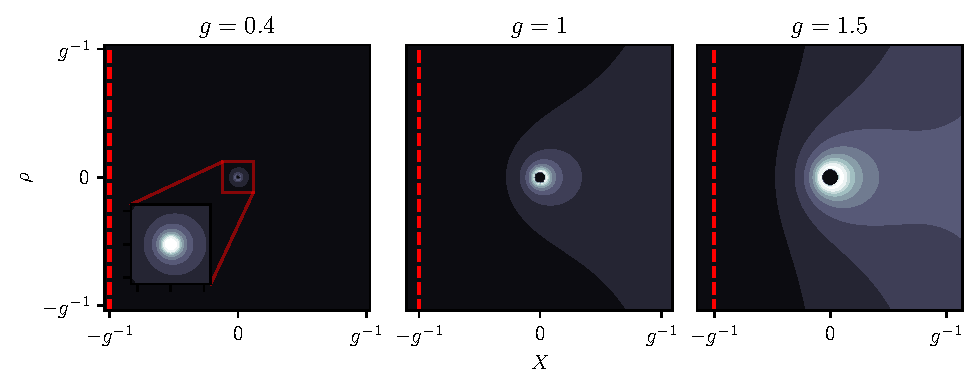
\includegraphics{C:/Users/pgraham1/Documents/GitHub/PSI/Relativity/Homework1/TeX-JAM/Equi_Sketch.pdf}
    \caption{$X, \rho$ Sketch of the equipotentials of the modified coulomb potential $\phi$ for different values of acceleration $g$. The red dashed lines represent the Rindler horizon located at $X=-1/g$. Negative values of $\rho$ were included for aesthetic purposes.}
    \label{equi}
  \end{figure}
  \item[(d)] Figure \ref{equi} represents equipotentials of the modified coulomb potential $\phi$. We notice that for small acceleration (see $g=0.4$ plot), the equipotentials resemble Coulomb's law and the horizon influence on the equipotential is reduced because it is far from the main region of influence of the point charge. for $g=1$ we start seeing the effect of proximity to the horizon opening the equipotentials. The $g=1.5$ plot suggests that equipotentials become parallel to the horizon for sufficient proximity of the charge to the Rindler horizon (equivalent to high acceleration). To make sense of this behavior, we notice that in the Rindler frame, the coordinate speed of light is not constant. Using the Rindler metric, we can write the coordinate speed of light as 
  \begin{align*}
    0 = -(1+gX)^2 dT^2 + dX^2 + \rho^2 d\varphi^2 + d\rho^2 \iff 1+gX = \sqrt{\left(\dfrac{dX}{dT}\right)^2 + \rho^2 \left(\dfrac{d\varphi}{dT}\right)^2 + \left(\dfrac{d\rho}{dT}\right)^2}  
  \end{align*}
  which differs from the usual $1$ obtained for Minkowski coordinate speed. Forgetting that we have accelerating observers, we can interpret this inhomogeneous speed of light as a modified electric permittivity of spacetime. The relative permitivity $\epsilon$ is related to the speed of light trough $1+gX = 1/\sqrt{\epsilon}$ implying $\epsilon = (1+gX)^{-2}$ in this dielectric analogy. This change in permittivity affects Maxwell's Gauss law introducing fictive bound charges. The equipotentials parallel to the Rindler horizon can be understood as arising from the field produced by these bound charges. There is a connection to make between this permittivity and the curved space Gauss law involving the determinant of the metric.

  \item[(e)]   In vacuum curved spacetime, the Gauss-Ampere law is expressed in terms of the electromagnetic tensor $F^{\mu\nu'}$ and the metric determinant $g$ as 
  \begin{align*}
    \dfrac{1}{\sqrt{-g}} \partial_\mu (\sqrt{-g} g^{\mu \alpha} g^{\nu \beta} F_{\alpha\beta'}) = 0.
  \end{align*}
  For the Rindler spacetime, we have $g = -(1+gX)^2 \times 1 \times 1 \times \rho^2$. Going back to the comment on permittivity, we notice that this equation (for $\nu =0$) can be written in terms of the electric field components covariant divergence $\nabla \cdot$ as 
  \begin{align*}
    \dfrac{1}{\sqrt{-g}} \nabla (\sqrt{-g} (1+gX)^{-2}\mathbf{E}) = \nabla \cdot (\epsilon \mathbf{E}) = 0
  \end{align*}
  which is exactly the covariant Gauss law with a special permittivity.\\
  
  
  In the gauge derived above, we directly see that the only nontrivial components of $F^{\mu\nu'}$ are $F^{X0'}, F^{\rho0'}$ and their transpose. They are given by 
  \begin{align*}
    &F_{X0'} = \frac{\partial \Phi}{\partial X} = - \frac{Q X \left(X g + \frac{g^{2} \left(X^{2} + \rho^{2}\right)}{2} + 1\right)}{\left(X^{2} + \rho^{2}\right)^{\frac{3}{2}} \sqrt{X g + \frac{g^{2} \left(X^{2} + \rho^{2}\right)}{4} + 1}} + \frac{Q \left(- \frac{X g^{2}}{4} - \frac{g}{2}\right) \left(X g + \frac{g^{2} \left(X^{2} + \rho^{2}\right)}{2} + 1\right)}{\sqrt{X^{2} + \rho^{2}} \left(X g + \frac{g^{2} \left(X^{2} + \rho^{2}\right)}{4} + 1\right)^{\frac{3}{2}}} + \frac{Q \left(X g^{2} + g\right)}{\sqrt{X^{2} + \rho^{2}} \sqrt{X g + \frac{g^{2} \left(X^{2} + \rho^{2}\right)}{4} + 1}},\\
    &F_{\rho0'} = \frac{\partial \Phi}{\partial \rho} = \frac{Q g^{2} \rho}{\sqrt{X^{2} + \rho^{2}} \sqrt{X g + \frac{g^{2} \left(X^{2} + \rho^{2}\right)}{4} + 1}} - \frac{Q g^{2} \rho \left(X g + \frac{g^{2} \left(X^{2} + \rho^{2}\right)}{2} + 1\right)}{4 \sqrt{X^{2} + \rho^{2}} \left(X g + \frac{g^{2} \left(X^{2} + \rho^{2}\right)}{4} + 1\right)^{\frac{3}{2}}} - \frac{Q \rho \left(X g + \frac{g^{2} \left(X^{2} + \rho^{2}\right)}{2} + 1\right)}{\left(X^{2} + \rho^{2}\right)^{\frac{3}{2}} \sqrt{X g + \frac{g^{2} \left(X^{2} + \rho^{2}\right)}{4} + 1}}
  \end{align*}
  calculated with 
  \begin{python}
EX = sp.diff(Phi, X)
Erho = sp.diff(Phi, rho)
EX.simplify()
Erho.simplify()
  \end{python}
Substituting the previous results in the right-hand side of the modified Maxwell equation stated above for $\nu = 0$ (only non-trivial components) we obtain $0$. The calculation was performed using the code 
\begin{python}
Maxwell = sp.diff(EX * rho/(1+g*X), X) + sp.diff(Erho * rho/(1+g*X), rho)
Maxwell.simplify()
    \end{python}


\end{enumerate}  

\section{Acknowledgement}
Thanks to Thomas for the interesting trick used to calculate the intersection of the hyperbolic trajectory and the light cone.\\

Thanks to Maitá, Nikhil, and Thomas for the interesting discussions about the dielectric interpretation of the equipotential deformation.\\ 

Thanks to Thiago for a discussion about the general definition of acceleration.



% References
\makereferences
%-------------------------------------------------------


%%%%%%%%%%%%%%%%%%%%%%%%
% Terminer le document %
%%%%%%%%%%%%%%%%%%%%%%%%
\end{document}